\documentclass[11pt]{article}
\usepackage[a4paper,margin=2.2cm]{geometry}
\usepackage{amsmath}
\usepackage{booktabs}
\usepackage{array}
\usepackage[table]{xcolor}
\usepackage{tikz}
\usetikzlibrary{positioning, arrows.meta, fit, backgrounds}
\usepackage[T1]{fontenc}
\setlength{\parindent}{0pt}
\setlength{\parskip}{4pt}

\definecolor{tealc}{RGB}{29,158,117}
\definecolor{coralc}{RGB}{216,90,48}
\definecolor{grayc}{RGB}{120,120,116}
\definecolor{lightbg}{RGB}{244,242,236}

\newcommand{\rms}{\mathrm{RMS}}

\begin{document}

\begin{center}
{\large\bfseries Rhythm-fidelity metrics for the Music-SDTB stimuli}\\[2pt]
the methods considered, the dimensions manipulated, and why one was kept
\end{center}

\vspace{2pt}

\section*{The question and one worked example}

We want a single index of how faithfully the rendered timing of a Beat sequence
matches its intended timing. Every method below is applied to the same toy
example, chosen so the methods separate cleanly. Nominal pulse period
$S = 100$~ms. The Beat marks pulses $0,1,4,5$ (silent at $2,3$); the recorded
onsets are
\[
  o_0 = 0,\quad o_1 = 120,\quad o_4 = 420,\quad o_5 = 520 \ \text{ms}.
\]
The whole error lives in the first interval: Standard~1 ($o_1-o_0 = 120$) is
rendered $+20\%$ long, while SOA~1 ($o_4-o_1 = 300$) and Standard~2
($o_5-o_4 = 100$) are perfect. How each method attributes that single error is
what distinguishes them.

\section*{Overview: the dimensions manipulated}

Two families. A metric either measures \emph{intervals} (each duration against
its own nominal, no shared reference) or measures \emph{onset positions} against
a common grid. The grid family then splits along two independent binary choices:
how the grid's \emph{phase} is set (pinned to the first onset, or fitted by least
squares) and what \emph{period} it uses (the nominal $S$, or a fitted tempo).
That is a $2\times2$ of grid methods, plus the single per-element method outside
it.

\begin{center}
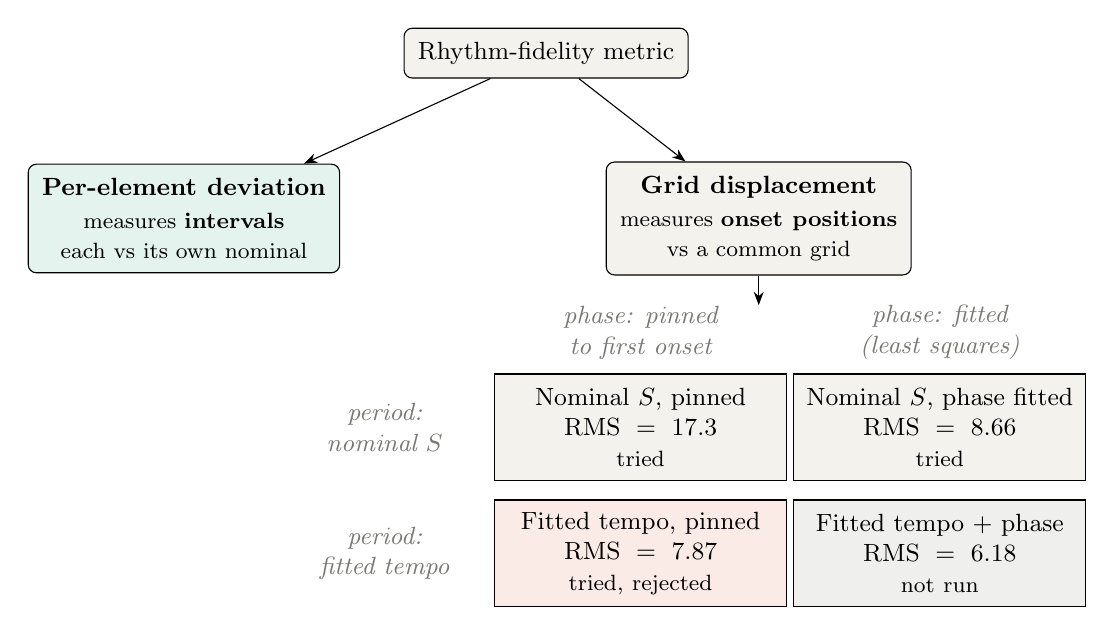
\begin{tikzpicture}[
  font=\small,
  box/.style={draw, rounded corners=3pt, align=center, inner sep=5pt},
  cell/.style={draw, align=center, inner sep=3pt, text width=3.5cm, minimum height=1.35cm},
  hdr/.style={align=center, font=\small\itshape, text=grayc},
  >=Stealth
]
\node[box, fill=lightbg] (root) at (1.6,0.2)
  {Rhythm-fidelity metric};

\node[box, fill=tealc!12] (pe) at (-3.0,-1.9)
  {\textbf{Per-element deviation}\\[1pt]\footnotesize measures \textbf{intervals}\\\footnotesize each vs its own nominal};
\node[box, fill=lightbg] (grid) at (4.3,-1.9)
  {\textbf{Grid displacement}\\[1pt]\footnotesize measures \textbf{onset positions}\\\footnotesize vs a common grid};

\draw[->] (root) -- (pe);
\draw[->] (root) -- (grid);

\node[hdr] at (2.8,-3.35) {phase: pinned\\to first onset};
\node[hdr] at (6.6,-3.35) {phase: fitted\\(least squares)};
\node[hdr, text width=1.7cm] at (-0.45,-4.55) {period:\\nominal $S$};
\node[hdr, text width=1.7cm] at (-0.45,-6.15) {period:\\fitted tempo};

\node[cell, fill=lightbg] (c11) at (2.8,-4.55)
  {Nominal $S$, pinned\\ $\rms = 17.3$\\ \footnotesize tried};
\node[cell, fill=lightbg] (c12) at (6.6,-4.55)
  {Nominal $S$, phase fitted\\ $\rms = 8.66$\\ \footnotesize tried};
\node[cell, fill=coralc!12] (c21) at (2.8,-6.15)
  {Fitted tempo, pinned\\ $\rms = 7.87$\\ \footnotesize tried, rejected};
\node[cell, fill=grayc!12] (c22) at (6.6,-6.15)
  {Fitted tempo + phase\\ $\rms = 6.18$\\ \footnotesize not run};

\draw[->] (grid) -- (4.3,-3.0);
\end{tikzpicture}
\end{center}

\emph{Reading it:} the left column pins the grid to the first onset (that event
gets residual~$0$); the right column places the grid by least squares (no event
privileged). The top row keeps the nominal period, so the residual is deviation
from the \emph{intended} timing; the bottom row fits the tempo, so the residual
is only the \emph{anisochrony} left after the rendered rate is removed. Per-element
sits outside this grid entirely.

\section*{Family 1 --- per-element deviation (the method kept)}

Each interval is compared with its own nominal, independently. For interval $i$
with rendered duration $d_i$ and nominal $n_i$, the deviation is $e_i = d_i-n_i$
(ms) or $p_i = 100(d_i-n_i)/n_i$ (\%). There is no shared timeline and no anchor,
so nothing propagates: on the example it reports the truth exactly --- Standard~1
$+20\%$, SOA~1 and Standard~2 $0\%$. The error stays where it happened.

\begin{center}
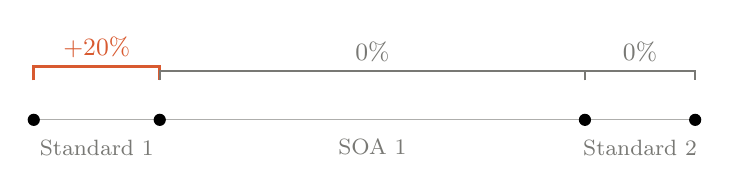
\begin{tikzpicture}[font=\small]
  \def\yb{0}
  \draw[grayc!60, line width=0.4pt] (0,\yb) -- (8.4,\yb);
  \foreach \x in {0,1.6,7.0,8.4} \fill (\x,\yb) circle (2.2pt);
  % Standard 1 bracket (error), coral
  \draw[coralc, line width=1.2pt] (0,\yb+0.5) -- (0,\yb+0.68) -- (1.6,\yb+0.68) -- (1.6,\yb+0.5);
  \node[coralc, font=\small] at (0.8,\yb+0.92) {$+20\%$};
  % SOA1
  \draw[grayc, line width=0.6pt] (1.6,\yb+0.5) -- (1.6,\yb+0.62) -- (7.0,\yb+0.62) -- (7.0,\yb+0.5);
  \node[grayc, font=\small] at (4.3,\yb+0.86) {$0\%$};
  % Std2
  \draw[grayc, line width=0.6pt] (7.0,\yb+0.5) -- (7.0,\yb+0.62) -- (8.4,\yb+0.62) -- (8.4,\yb+0.5);
  \node[grayc, font=\small] at (7.7,\yb+0.86) {$0\%$};
  \node[font=\footnotesize, text=grayc] at (0.8,\yb-0.35) {Standard 1};
  \node[font=\footnotesize, text=grayc] at (4.3,\yb-0.35) {SOA 1};
  \node[font=\footnotesize, text=grayc] at (7.7,\yb-0.35) {Standard 2};
\end{tikzpicture}
\end{center}

The output is one number per element kind (Standard, SOA, and the two pooled),
per modality, condition, and task. Its reference is local, so it is the only
method that needs no choice of anchor or tempo. This is the metric now in the
script and the paper.

\section*{Family 2 --- grid displacement (four variants)}

Here each onset is measured against a line $o_k \approx a + b\,k$ over pulse index
$k$, where $b$ is the period and $a$ the phase. The figure (next page) plots each
onset as its offset from the nominal grid, $o_k - S k$ (so the toy points are
$0,20,20,20$ at $k=0,1,4,5$); each method is then a reference line, and the
residual is the vertical gap. A \emph{horizontal} line means the period stayed
nominal; a \emph{tilted} line means the tempo was fitted. A line \emph{through the
first point} is pinned; one placed elsewhere is phase-fitted.

\clearpage
\section*{Family 2 --- the four grid fits on the worked example}

\begin{center}
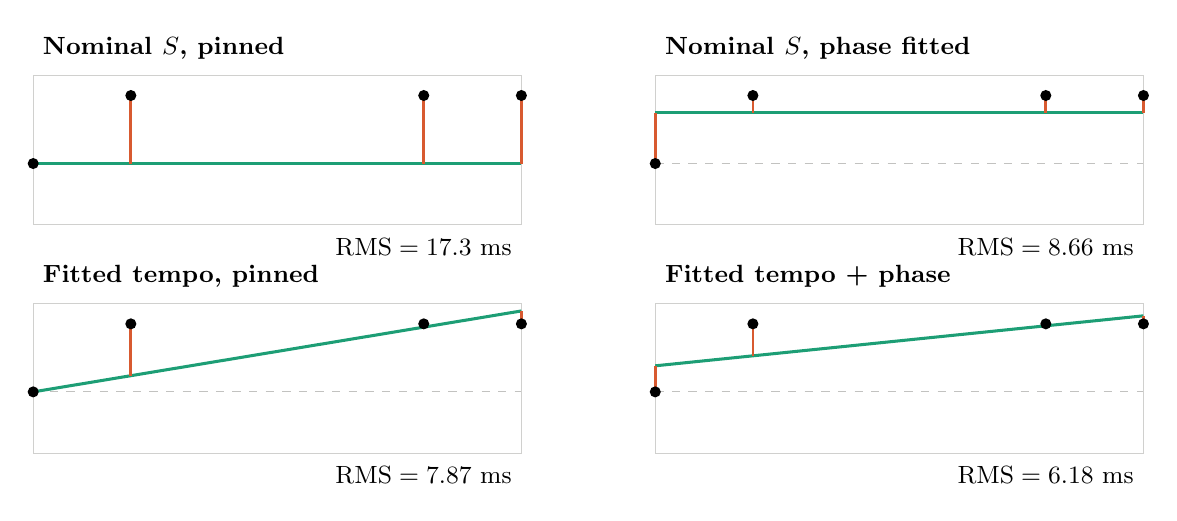
\begin{tikzpicture}[font=\small]

\newcommand{\subplot}[5]{%
  \begin{scope}[shift={(#1,#2)}]
    \draw[grayc!35, line width=0.4pt] (0,0) rectangle (6.2,1.9);
    \draw[grayc!45, dashed, line width=0.3pt] (0,0.777) -- (6.2,0.777);
    \node[anchor=south west, font=\small\bfseries] at (0,1.98) {#3};
    \node[anchor=north east, font=\small] at (6.2,-0.05) {$\rms = #4$~ms};
    #5
    \foreach \px/\py in {0/0.777, 1.24/1.641, 4.96/1.641, 6.2/1.641}
      \fill (\px,\py) circle (2.0pt);
  \end{scope}
}

% x scale: k*1.24 (k in 0..5 -> 0..6.2). y=(off+18)/44*1.9.
% TL nominal pinned: ref horizontal at 0.777; residuals to it
\subplot{0}{2.9}{Nominal $S$, pinned}{17.3}{%
  \draw[tealc, line width=1.1pt] (0,0.777) -- (6.2,0.777);
  \draw[coralc, line width=1.0pt] (1.24,1.641) -- (1.24,0.777);
  \draw[coralc, line width=1.0pt] (4.96,1.641) -- (4.96,0.777);
  \draw[coralc, line width=1.0pt] (6.2,1.641) -- (6.2,0.777);
}
% TR nominal phase: ref horizontal at off=15 -> y=(33/44)*1.9=1.425
\subplot{7.9}{2.9}{Nominal $S$, phase fitted}{8.66}{%
  \draw[tealc, line width=1.1pt] (0,1.425) -- (6.2,1.425);
  \draw[coralc, line width=1.0pt] (0,0.777) -- (0,1.425);
  \draw[coralc, line width=1.0pt] (1.24,1.641) -- (1.24,1.425);
  \draw[coralc, line width=1.0pt] (4.96,1.641) -- (4.96,1.425);
  \draw[coralc, line width=1.0pt] (6.2,1.641) -- (6.2,1.425);
}
% BL fitted tempo pinned: ref from (0,0.777) to off=23.8 -> y=(41.8/44)*1.9=1.805
% line value: y=0.777+(1.805-0.777)/6.2 * x = 0.777+0.1658x
\subplot{0}{0}{Fitted tempo, pinned}{7.87}{%
  \draw[tealc, line width=1.1pt] (0,0.777) -- (6.2,1.805);
  \draw[coralc, line width=1.0pt] (1.24,1.641) -- (1.24,0.983);
  \draw[coralc, line width=1.0pt] (4.96,1.641) -- (4.96,1.599);
  \draw[coralc, line width=1.0pt] (6.2,1.641) -- (6.2,1.805);
}
% BR fitted tempo + phase: off=7.65 at k0 -> y=(25.65/44)*1.9=1.108; off=22.35 k5 -> y=1.743
% line: y=1.108+(1.743-1.108)/6.2 x = 1.108+0.1024x
\subplot{7.9}{0}{Fitted tempo + phase}{6.18}{%
  \draw[tealc, line width=1.1pt] (0,1.108) -- (6.2,1.743);
  \draw[coralc, line width=1.0pt] (0,0.777) -- (0,1.108);
  \draw[coralc, line width=1.0pt] (1.24,1.641) -- (1.24,1.235);
  \draw[coralc, line width=1.0pt] (4.96,1.641) -- (4.96,1.617);
  \draw[coralc, line width=1.0pt] (6.2,1.641) -- (6.2,1.743);
}
\end{tikzpicture}
\end{center}

\vspace{2pt}
{\footnotesize
Black dots: each onset as its offset $o_k - Sk$ from the nominal grid.
\textcolor{tealc}{Teal}: the method's reference grid. \textcolor{coralc}{Coral}:
the residual (vertical gap). Dashed gray: the nominal grid ($o_k - Sk = 0$).}

\vspace{6pt}

\textbf{Nominal $S$, pinned.} Period held at $S$; the line passes through the
first onset, whose residual is therefore $0$ by construction. Because every later
interval is perfect, the first interval's $+20$ carries forward and all later
onsets read $+20$: a single early error becomes a displacement of the whole
sequence. Residuals $0,+20,+20,+20$; $\rms = 17.3$~ms.

\textbf{Nominal $S$, phase fitted.} Period held at $S$; the phase
$c=\text{mean}(o_k-Sk)=15$ is fitted, so no onset is privileged. The fit sees the
sequence as consistently $+15$ with $o_0$ the outlier. Residuals
$-15,+5,+5,+5$; mean zero; $\rms = 8.66$~ms.

\textbf{Fitted tempo, pinned} (the original \texttt{"fitted"} method). The line
still passes through the first onset, but the slope --- the period --- is fitted,
giving the rendered tempo $104.8$~ms ($+4.8\%$). The residual is the anisochrony:
what remains after that constant tempo is removed. The $+20$ splits between the
tempo and the residual. Residuals $0,+15.2,+0.95,-3.81$; $\rms = 7.87$~ms.

\textbf{Fitted tempo + phase.} Both slope and phase fitted (ordinary least
squares); no constraint. Residuals $-7.65,+9.41,+0.59,-2.35$; $\rms = 6.18$~ms.
The logical fourth corner; not run.

\section*{Summary and why per-element was kept}

\begin{center}
\renewcommand{\arraystretch}{1.25}
\footnotesize
\begin{tabular}{@{}p{3.2cm} p{2.2cm} p{3.0cm} p{2.6cm} c@{}}
\toprule
\textbf{Method} & \textbf{Measures} & \textbf{Reference} &
\textbf{Residuals, ms} & \textbf{RMS} \\
\midrule
Per-element & intervals & each own nominal & Std1 $+20$; rest $0$ & --- \\
Nominal $S$, pinned & onset positions & grid $\perp S$, through 1st onset & $0,20,20,20$ & $17.3$ \\
Nominal $S$, phase fit & onset positions & grid $\perp S$, phase $=$ LSQ & $-15,5,5,5$ & $8.66$ \\
Fitted tempo, pinned & onset positions & slope $=$ tempo, through 1st onset & $0,15.2,0.95,-3.8$ & $7.87$ \\
Fitted tempo + phase & onset positions & slope + phase $=$ LSQ & $-7.7,9.4,0.6,-2.4$ & $6.18$ \\
\bottomrule
\end{tabular}
\end{center}

RMS falls monotonically as parameters are freed ($17.3 \to 8.66$ or
$7.87 \to 6.18$), but smaller is not better: each freed parameter removes
something from the residual, and freeing the tempo changes what the number
\emph{means} (anisochrony from the rendered rate, rather than deviation from the
intended timing). The fitted-tempo row assumes the listener entrains to whatever
rate was rendered, so a uniform tempo offset is not counted as error --- the
assumption we rejected, which is what removed the original \texttt{"fitted"}
method. The nominal-period row keeps the intended timing as reference, but the
grid still couples the onsets, and the pinned version inherits whatever the first
onset did. Per-element drops the grid altogether: no anchor, no tempo, no
coupling; each interval against its own nominal, error kept local. Having tried
the four grid variants, the analysis ended on the per-element deviation.

\end{document}
